\chapter{Iteracion 4: Diseño final del Software} % (fold)
\label{cha:iteracion_4}

\section{Introduccion} % (fold)
\label{it5:sec:introduccion}

En esta iteracion, se intentó dar un cierre a un primer prototipo de software que cumpla con todos los requerimientos, o la mayor cantidad posible, teniendo en cuenta el riesgo intrinseco de cada uno.

Al final de la iteracion 2, en la seccion \ref{it2:sec:conclusiones_de_la_iteracion_2}, se especifica una lista con requerimientos cumplidos. Nuestro punto de partida para continuar el desarrollo del programa es esta lista. 

El objetivo principal de esta iteracion es conformar un programa que cumpla con todos los requerimientos inherentes al software de la plataforma.

% section introduccion (end)

\section{Requerimientos de la iteracion} % (fold)
\label{it5:sec:requerimientos_de_la_iteracion}

Los requerimientos de esta iteracion estan planteados en base a los resultados de las pruebas y el desarrollo de la iteracion 2. 

\begin{itemize}
\item Se deberian poder configurar tiempos de intervalo entre cada medicion para cada canal por separado
\item Se deberian poder guardar las configuraciones actuales en la memoria flash del microcontrolador, para poder reestablecerlas en caso que el sistema se apague y se vuelva a prender.
\item Se deberia generar una marca de tiempo relativa al inicio de conversiones en cada medicion realizada.
\item Los datos que se envian a la placa de gestion para cada medicion deberia inculir, ademas de la medicion, el numero de pin o pines (si es modo diferencial) de donde se esta midiendo. 
\item Los datos que se envian a la placa de gestion para cada medicion deberia inculir, ademas de la medicion, el modo de conversion del canal por donde se esta midiendo.
\item Los datos que se envian a la placa de gestion para cada medicion deberia inculir, ademas de la medicion, la marca de tiempo relativa correspondiente de la medicion hecha. 
\end{itemize}


% section requerimientos_de_la_iteracion (end)

\section{Desarrollo} % (fold)
\label{it5:sec:desarrollo}

Focalizamos el desarrollo del programa en obtener un prototipo final, preparado para que se ejecute de manera continua en la placa de instrumentacion construida. En una primera instancia, terminamos aquellas funcionalidades ligadas a los requerimientos principales, y luego nos dedicamos a comprobar el funcionamiento del mismo, mediante unit-testing y tests de sistema.

La figura \ref{it5:fig:bloquesquintaiteracion} muestra el diagrama de bloques del programa terminado, al final esta iteracion. Si se compara con la figura \ref{it2:fig:bloquesprimeraiteracionsoftware}, el cambio en la estructura no es significativo. El mayor cambio esta en las funciones dentro de los bloques. Hay funciones nuevas, funciones que sufrieron cambios y funciones que se eliminaron.

\begin{figure}[h]
  \centering
  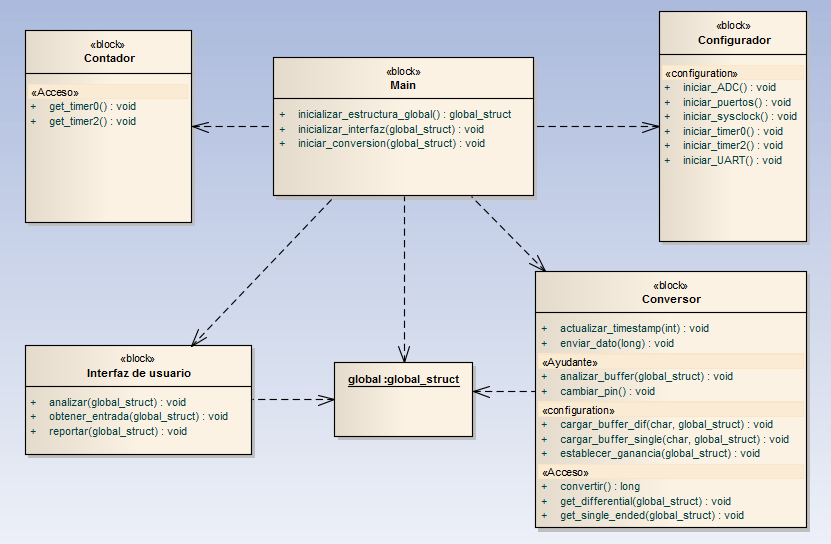
\includegraphics[width=0.80\textwidth, height = 9cm]{bloquesquintaiteracion}
  \caption{}\label{it5:fig:bloquesquintaiteracion}
\end{figure}

\subsection{Conversor} % (fold)
\label{sub:conversor}

Las funciones del conversor se rediseñaron con el objetivo de lograr que el usuario pueda configurar tiempos de intervalos de mediciones en cada canal por separado.

En la seccion \ref{it2:sub:el_modulo_conversor}, se explica el funcionamiento del buffer del conversor. Hasta el momento, el buffer poseia 8 posiciones, una por cada canal, con el objetivo de informar al programa el estado de ese canal. Estos estados son: inhabilitado, canal unico, o canal diferencial.

\begin{figure}[h]
  \centering
  \includegraphics[width=0.80\textwidth, height = 7cm]{bufferdinamicovacio}
  \caption{Estado de los buffers en el momento en que se terminaron de configurar las distintas vias de conversion, pero aun no se activo el modo de conversion continua}\label{it5:fig:bufferdinamicovacio}
\end{figure}

En esta version del programa, utilizamos dos buffers de 11 posiciones cada uno. A diferencia del buffer de conversion de la iteracion 2, cada posicion ya no representa un unico canal sino que representa una "via de conversion". Una via de conversion es una fuente de telemetria que puede provenir de un canal unico o diferencial.
De manera figurativa, podria decirse que un buffer es "dinamico", y el otro es "estatico". Similar al buffer de conversion de la iteracion 2, el buffer estatico determina si un canal esta habilitado o no. Ademas de esto, determina el valor del intervalo de mediciones de dicho canal. Si la posicion que corresponde a ese canal contiene un 0, el canal esta inhabilitado; cualquier numero mayor a 0 indica que el canal esta habilitado. Si el canal esta habilitado, el numero puede estar en un rango de 1 a 65536, siendo este numero una medida del intervalo temporal que habra entre cada medicion cuando el sistema entre en modo de conversiones continuas. Mientras mayor es el numero, mayor es el intervalo entre cada medicion para ese canal.
A diferencia del buffer original, el modo de conversion ya no se identifica con un numero, sino con la posicion dentro del buffer, ya sea el estatico o el dinamico. Las posiciones del 0 al 7 estan reservadas para los 8 canales del conversor en modo canal unico, y las posiciones del 8 al 11 son para los canales en modo diferencial. Las posiciones 8,9,10 y 11 representan a los pares de pines en modo diferencial (1,2); (3,4); (5,6) y (7,8) respectivamente. 


La secuencia para las conversiones funciona de la siguiente manera:

\begin{enumerate}
\item Cuando se configura el buffer, se establecen las vias de conversion con sus respectivos intervalos poniendo numeros de 1 a 65536 en los elementos del buffer estatico.
\item Cuando se activa el modo de conversiones continuas, se realiza una copia del buffer estatico para obtener el buffer dinamico, que es en realidad una instancia del buffer estatico al comienzo de la conversiones continuas.
\item El programa itera sobre el buffer dinamico, decrementando los valores de cada elemento del buffer que no contenga un 0
\item Cuando se encuentra sobre un elemento que tiene valor igual a 1, es momento de obtener una medicion de la via de conversion ligada a esa posicion.
\item Una vez habilitada la conversion para el canal, se copia el valor que se encuentra en el buffer estatico para la misma posicion en el buffer dinamico. Reiniciando la cuenta.
\end{enumerate}

La funcion que realiza la conversion, es ejecutada cada vez que se encuentra un 1 en una posicion del buffer dinamico. Con el numero de posicion del buffer, se sabe el numero de la via de conversion por donde hay que convertir. Esta via de conversion, como mencionamos anteriormente, puede ser de 0 a 11. En cada numero, se mide lo siguiente:

\begin{itemize}
\item 0 \textrightarrow  canal 0 modo unico
\item 1 \textrightarrow  canal 1 modo unico
\item 2 \textrightarrow  canal 2 modo unico
\item 3 \textrightarrow  canal 3 modo unico
\item 4 \textrightarrow  canal 4 modo unico
\item 5 \textrightarrow  canal 5 modo unico
\item 6 \textrightarrow  canal 6 modo unico
\item 7 \textrightarrow  canal 7 modo unico
\item 8 \textrightarrow  canal 0,1 modo diferencial
\item 9 \textrightarrow  canal 1,2 modo diferencial
\item 10 \textrightarrow  canal 2,3 modo diferencial
\item 11 \textrightarrow  canal 3,4 modo diferencial
\end{itemize}

Se tomaron las medidas suficientes, dentro del programa, para no permitir al usuario que establezca una configuracion donde provoque que se solapen las vias de conversion con respecto a los canales. 

\begin{figure}[h]
  \centering
  \includegraphics[width=0.80\textwidth, height = 7cm]{bufferdinamicolleno}
  \caption{Estado de los buffers en el momento que se activa la conversion continua. Cada vez que un valor del buffer dinamico llega a 1, se reestablece usando el buffer estatico como referencia.}\label{it5:fig:bufferdinamicolleno}
\end{figure}

El numero dentro de cada posicion representa el tiempo del intervalo. El intervalo mas corto es 1, y el mas largo es 65536. Los tiempos en segundos con respecto a los intervalos siguen una escala que tiende a ser lineal, pero necesaria de calibrar en caso de ser necesaria una meyor presicion. Para mejorar la practicidad a la hora de establecer intervalos, conformamos una tabla con valores de intervalos nominales. A partir de dicha tabla, elabramos un grafico que se muestra en la figura \ref{it5:fig:relacionintervalotiempo}.

\begin{table}[h]
\centering
\caption{Tabla con mediciones de tiempo para distintos valores de intervalos.}
\label{it5:tab:tablamediciones}
\begin{tabular}{|l|l|}
\hline
\rowcolor[HTML]{34CDF9} 
Intervalo & Tiempo (s) \\ \hline
\rowcolor[HTML]{CBF3FF} 
9         & 1          \\ \hline
\rowcolor[HTML]{CBF3FF} 
28        & 3          \\ \hline
\rowcolor[HTML]{CBF3FF} 
55        & 6          \\ \hline
\rowcolor[HTML]{CBF3FF} 
92        & 10         \\ \hline
\rowcolor[HTML]{CBF3FF} 
138       & 15         \\ \hline
\end{tabular}
\end{table}

\begin{figure}[h]
  \centering
  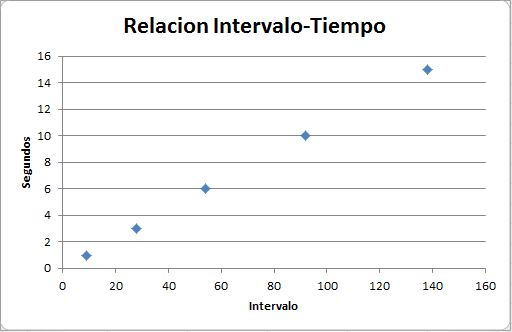
\includegraphics[width=0.80\textwidth, height = 7cm]{relacionintervalotiempo.JPG}
  \caption{Grafico Grafico elaborado a partir de la tabla \ref{it5:tab:tablamediciones}}[Grafico elaborado a partir de la tabla \ref{it5:tab:tablamediciones}, obtenidos midiendo el tiempo entre cada medicion para los intervalos en el eje de las abscisas. Observando la curva, llegamos a la conclusion del que los distintos valores de tiempo correspondientes a los intervalos se comportan de manera lineal. Haciendo una extrapolacion basica, podemos decir que el intervalo mas largo, con un valor de 65536, corresponde a un tiempo de aproximadamente 2 horas entre cada medicion.]\label{it5:fig:relacionintervalotiempo}
\end{figure}

Las funciones "cambiar\_pin" y "analizar\_buffer" dentro del modulo de conversor, manejan los buffers y realizan las conversiones segun las configuraciones. Ambas son ejecutadas ciclicamente en el modo de conversiones continuas. "cambiar\_pin" prepara el hardware del conversor segun cual es el canal proximo a medir, y "analizar\_buffer" recorre el buffer, habilitando o no la conversion, y actualizandolo en cada corrida. Las figuras \ref{it5:fig:actividadanalizarbuffer} y \ref{it5:fig:actividadcambiarpin} describen las funciones con diagramas de actividad.
 
\begin{figure}[h]
  \centering
  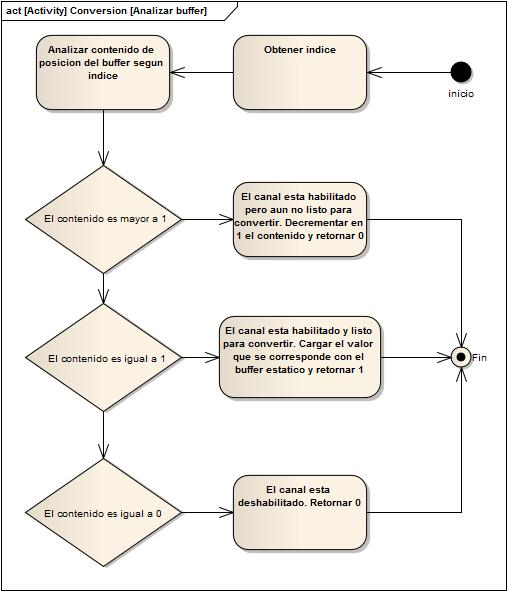
\includegraphics[width=0.80\textwidth, height = 7cm]{actividadanalizarbuffer}
  \caption[Diagrama de actividad de la funcion analizar buffer]{Diagrama de actividad que muestra el funcionamiento de la funcion analizar buffer. Esta funcion esta pensada para trabajar junto con "cambiar\_pin". En cada cambio de pin, se analiza el buffer para saber si hay que convertir o no, y actualizar el estado de los elementos del buffer, que corresponden en uno a uno con todas las vias de conversion posibles.}\label{it5:fig:actividadanalizarbuffer}
\end{figure}



\begin{figure}[h]
  \centering
  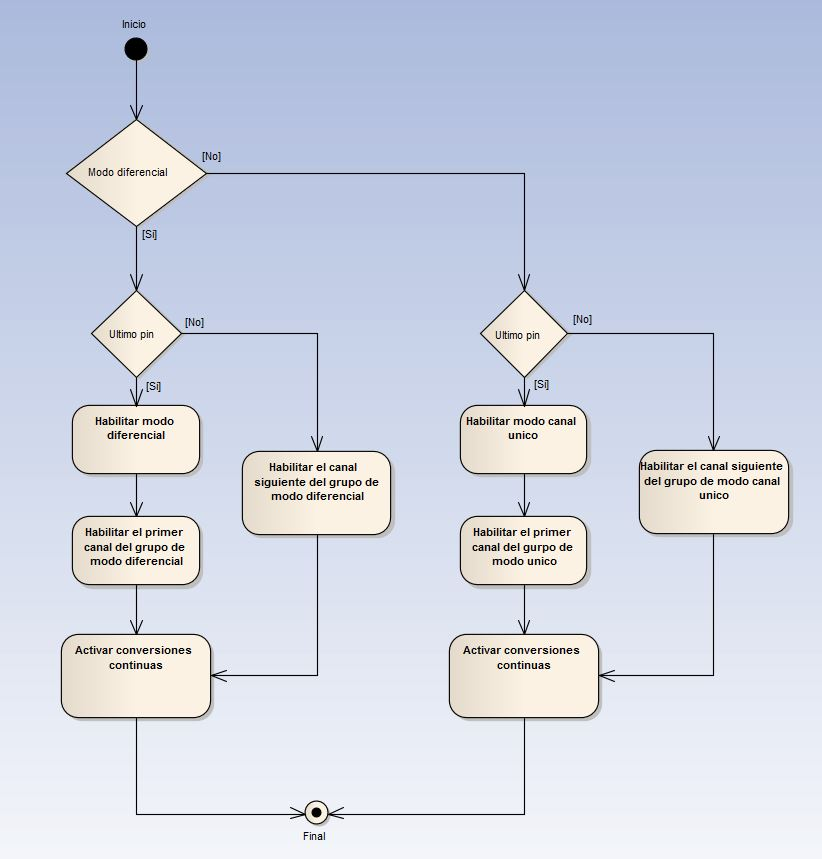
\includegraphics[width=0.80\textwidth, height = 7cm]{actividadcambiarpin}
  \caption[Diagrama de actividad de la funcion cambiar pin]{Diagrama de actividad que ilustra la logica dentro de la funcion cambiar\_pin, dentro del modulo del conversor. Esta funcion es llamada luego de cada conversion. En cada llamado, se selecciona un nuevo canal a medir. No discrimina si el canal esta o no habilitado para medir, en caso en que no lo este, se llamara inmediatamente para cambiar el pin nuevamente sin realizar medicion alguna.}\label{it5:fig:actividadcambiarpin}
\end{figure}

\subsubsection{Marca de tiempo} % (fold)
\label{ssub:marca_de_tiempo}

En algunos casos, puede ser necesario saber la hora, minuto y segundo en el que se midió. Para esto, sugerimos la idea de que se incluya una marca de tiempo dentro de los meta-datos enviados a la placa de gestion. Fue un requerimiento propuesto por nosotros en una etapa ya avanzada del proyecto. Esta marca de tiempo es necesariamente relativa al momento de inicio de conversiones continuas. Esto se debe a que la placa de instrumentacion no tiene manera directa de calcular la fecha y hora exacta del dia, por lo que obtener una marca de tiempo absoluta de manera directa en esta placa no es practico. 
La solucion planteada para obtener una marca de tiempo absoluta fue calculandola en la placa de gestion. Al estar esta placa conectada a internet, puede obtener facilmente la fecha y hora de inicio de conversiones. Con esto, a la fecha y hora se le suma la marca relativa de cada medicion, y se obtiene asi la marca de tiempo absoluta. Sabiendo esto, en esta seccion explicamos la obtencion de la marca de tiempo relativa. La obtencion de la marca de tiempo absoluta se obtiene usando la marca relativa junto con la fecha y hora actuales. Implica que debera calcularse en un sistema con posibilidad de obtener esta informacion \\

El proceso para obtener la marca de tiempo esta descripto en la imagen \ref{it5:fig:secuenciaobtenermarca} mediante un diagrama de secuencia. La marca de tiempo relativa se obtiene con el uso del timer2. Esto significa reducir la cantidad de contadores de eventos disponibles de 2 a 1, lo cual afecta de manera directa a un requerimiento principal. La solucion planteada fue dejar como opcional el calculo del timestamp, pudiendo asi elegir el uso del timer2 entre contador de eventos o contador interno para la marca de tiempo. Esto es posible porque hay casos donde no es necesario ser preciso a la hora de tener el tiempo de las mediciones, y se pueden calcular las marcas directamente desde el sistema de gestion, y asi dejar libre al timer2 para el conteo de eventos. Esto fue un compromiso dado el estado avanzado del proyecto.


\begin{figure}[h]
  \centering
  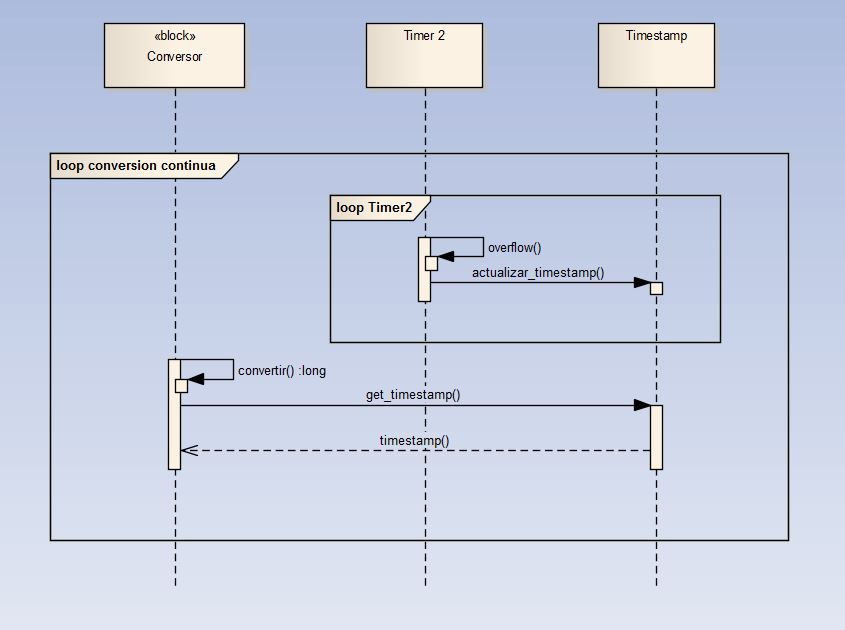
\includegraphics[width=0.80\textwidth, height = 7cm]{secuenciaobtenermarca}
  \caption[Diagrama de secuencia para la obtencion de una marca de tiempo]{Diagrama de secuencia que muestra la interaccion entre el conversor y timer 2 para obtener la marca de tiempo. En el diagrama, la marca de tiempo esta representada mediante un objeto que alberga un unico campo, que es la marca de tiempo. En cada interrupcion de Timer 2 este valor se actualiza, y en cada conversion se obtiene el valor actual para enviarlo junto con la medicion obtenida en la conversion.}\label{it5:fig:secuenciaobtenermarca}
\end{figure}

% subsubsection marca_de_tiempo (end)

% subsection conversor (end)

\subsection{Interfaz de usuario} % (fold)
\label{it5:sub:interfaz_de_usuario}

La interfaz de usuario siguio un diseño parecido al descripto en la seccion \ref{it2:sub:logica_de_las_funciones_de_la_interfaz}. Gracias al diseño de la interfaz, agregar nuevos comandos con nuevos argumentos era facil siempre y cuando se respetara la expresion regular.

Los comandos disponibles al final de esta iteracion fueron:

\begin{itemize}
  \item SSE: - \textit{set single ended}: Establece un canal en modo unico.
  \item SDI: - \textit{set differential}: Establece un par de canales en modo diferencial.
  \item GSE: - \textit{get single ended}: Obtiene una conversion instantanea en modo canal unico sobre un canal.
  \item GDI: - \textit{get differential}: Obtiene una conversion instantanea en modo diferencial sobre un par de canales.
  \item GDI: - \textit{get differential}: Obtiene una conversion instantanea en modo diferencial sobre un par de canales.
  \item SGA: - \textit{set gain}: Establece el nivel de ganancia del conversor.
  \item GT0: - \textit{get timer 0}: Obtiene el valor actual de la cuenta de timer 0, configurado como contador de eventos.
  \item GT2: - \textit{get timer 2}: Obtiene el valor actual de la cuenta de timer 2, configurado como contador de eventos.
  \item SHA: - \textit{show configuration}: Muestra la configuracion actual de todos los canales y la ganancia del conversor.
  \item ST: - \textit{start}: Inicia el modo de conversiones continuas.
\end{itemize}

El conjunto entero de comandos esta documentado con mayor detalle en el apendice \ref{ap:instrucciones}.
% subsection interfaz_de_usuario (end)

\subsection{Memoria flash} % (fold)
\label{it5:sub:memoria_flash}

La memoria flash del microcontrolador puede ser utilizada para guardar las configuraciones actuales, de forma que si el sistema se apaga, se pueda volver a iniciar con las configuraciones ya cargadas, sin necesidad de volver a establecer todo cada vez que se inicie nuevamente. Esto fue planteado como requerimiento para esta iteracion, pero no pudo ser posible. Las operaciones necesarias para leer y escribir la memoria y el tamaño de la misma hicieron que sea difícil realizar la escritura y la lectura de la misma.

Tanto el programa que corre en el microprocesador como los datos de configuración debe guardarse en la misma memoria flash de 8Kb, siendo que el programa ocupa alrededor de 7Kb. En el Kb que resta, es posible guardar las configuraciones, pero el método de escritura de la flash pone en riesgo la integridad del programa. La unica manera de escribir en memoria es haciendolo sobre una pagina de 512 bytes. Dado el reducido espacio disponible, era probable que en una escritura se sobreescribiera parte del programa, haciendo que el sistema falle.
Teniendo en cuenta esto, se decidió no utilizar la flash para guardar las configuraciones. Por lo tanto, cada vez que el sistema se apague, se pierden las configuraciones, sin posibilidad de guardarlas.

% subsection memoria_flash (end)

% section desarrollo (end)

\section{Pruebas} % (fold)
\label{it5:sec:pruebas}

\begin{table}[h]
\centering
\caption{Test de sistema 1}
\label{it5:tab:testsistema1}
\begin{tabular}{p{2cm} p{9cm}}
\multicolumn{2}{c}{\cellcolor[HTML]{68CBD0}{\color[HTML]{000000} Prueba de sistema}} \\
Prueba \#        & 3 \\
\hline
Nombre           & Comportamiento esperado del conversor \\
\hline
Requerimiento & Se deberian poder configurar tiempos de intervalo entre cada medicion para cada canal por separado. \\
\hline
Descripcion      & Con este test, se comprueba que el sistema permite establecer intervalos de medicion individuales para cada canal, y que se comporta de manera consistente con el el paso del tiempo. \\
\hline
Pre-condiciones  & \tabitem Sistema configurado con dos pines en modo canal unico \\
                 & \tabitem Un canal esta configurado con un tiempo de 1 y otro con 50 \\
                 & \tabitem Generadores de tension conectados a los pines configurados  \\
                 & \tabitem Computadora conectada al sistema mediante cable serial RS-232 \\
                 & \tabitem Lector de canal serial abierto en la computadora  \\
                 & \tabitem Sistema midiendo en modo de conversiones continuas\\
\hline

Post-condiciones & La frecuencia de medicion para el canal en 1 deberia ser mayor a la frecuencia del canal en 50.                     
\\
\hline
Secuencia  & \tabitem Establecimos una tension de 1,5 voltios en el primer generador, conectado al canal con intervalo 1 y una de 2 voltios en el segundo, con intervalo 50 \\
\hline
Resultados       & El canal con intervalo 1 tenia una frecuencia mucho mayor al canal con intervalo 50, que era lo esperado. La relacion entre las frecuencias parecia ser lineal (50 veces mas frecuente el primero que el segundo), aunque no teniamos una manera precisa de medirlo, mas que contar la cantidad de mediciones en un intervalo grande de tiempo.
\end{tabular}
\end{table}

\begin{table}[h]
\centering
\caption{Test de sistema 2}
\label{it5:tab:testsistema2}
\begin{tabular}{p{2cm} p{9cm}}
\multicolumn{2}{c}{\cellcolor[HTML]{68CBD0}{\color[HTML]{000000} Prueba de sistema}} \\
Prueba \#        & 3 \\
\hline
Nombre           & Generacion de la marca de tiempo \\                 
\hline
Requerimiento & Se deberia generar una marca de tiempo relativa al inicio de conversiones en cada medicion realizada. \\
\hline
Descripcion      & En cada conversion, se deberia registrar una marca de tiempo con un numero que hace referencia al tiempo que transcurrio desde el momento que se iniciaron las conversiones al momento donde se toma la medicion. \\
\hline
Pre-condiciones  & \tabitem Sistema configurado con un pin en modo canal unico, con un intervalo de 9, que corresponde a 1 segundo segun la tabla \ref{it5:tab:tablamediciones} \\
                 & \tabitem Generador de tension conectado al pin configurado  \\
                 & \tabitem Computadora conectada al sistema mediante cable serial RS-232 \\
                 & \tabitem Lector de canal serial abierto en la computadora  \\
                 & \tabitem Cronometro en 00:00\\
                 & \tabitem Reloj en hora\\
\hline

Post-condiciones & La diferencia entre cada marca de tiempo y la siguiente deberia ser constante, y deberia ser aproximada al valor en segundos dado por el intervalo. El calculo en fecha y hora de la ultima marca de tiempo y el valor del cronometro (hecho con ayuda del reloj) deberia dar aproximadamente igual. \\
\hline
Secuencia  & \tabitem Establecimos una tension en el generador. \\
           & \tabitem Iniciamos las conversiones continuas. \\
           & \tabitem Dimos arranque al cronometro. \\
           & \tabitem Medimos el tiempo entre cada medicion con ayuda del cronometro en 30 mediciones sucesivas. \\

Resultados       & Los resultados fueron los esperados. El intervalo de tiempo entre cada medicion era aproximadamente 1 segundo en todos los casos. Lo que significa que el tiempo entre cada medicion no varia con el paso del tiempo para un intervalo constante. 
\end{tabular}
\end{table}

\begin{table}[h]
\centering
\caption{Test de sistema 3}
\label{it5:tab:testsistema3}
\begin{tabular}{p{2cm} p{9cm}}
\multicolumn{2}{c}{\cellcolor[HTML]{68CBD0}{\color[HTML]{000000} Prueba de sistema}} \\
Prueba \#        & 3 \\
\hline
Nombre           & Formato esperado del mensaje \\                     
\hline
Requerimiento    & \tabitem Los datos que se envian a la placa de gestion para cada medicion deberia inculir, ademas de la medicion, el numero de pin o pines (si es mododiferencial) de donde se esta midiendo.  \\
                 & \tabitem Los datos que se envian a la placa de gestion para cada medicion deberia inculir, ademas de la medicion, el modo de conversion del canal por donde se esta midiendo. \\
                 & \tabitem Los datos que se envian a la placa de gestion para cada medicion deberia inculir, ademas de la medicion, la marca de tiempo relativa correspondiente de la medicion hecha. \\ 
\hline
Descripcion      & Cada dato que se envia a la placa de gestion incluye la siguiente informacion: Medicion, pin, modo, marca de tiempo. Estos datos estan enviados con un formato especial, y se envian en simultaneo. Esta prueba verifica que cada mensaje contenga el formato correcto y que los datos sean coherentes a las configuraciones. \\
\hline
Pre-condiciones  & \tabitem Sistema configurado con el pin 3 en modo canal unico, con un intervalo de 10 \\
                 & \tabitem Generador de tension conectado al pin configurado con un valor de 1,5 volts  \\
                 & \tabitem Computadora conectada al sistema mediante cable serial RS-232 \\
                 & \tabitem Lector de canal serial abierto en la computadora  \\
                 & \tabitem Sistema midiendo en modo de conversiones continuas\\
\hline

Post-condiciones & El mensaje recibido en el lector serial deberia ser "1500,3,SE,[marca de tiempo]".                     
\\
\hline
Resultados       & El formato era correcto
\end{tabular}
\end{table}

% section pruebas (end)

\section{Conclusiones} % (fold)
\label{sec:conclusiones}

Algunos de los requerimientos principales y secundarios no se llegaron a cumplir por inconvenientes en el desarrollo, pero se tomaron ciertas medidas para compensar los problemas, sobretodo en aquellos que involucraban a los requerimientos principales y de mayor riesgo.

\begin{itemize}
\item Guardar las configuraciones y parametros del programa en la memoria flash no fue posible debido al poco espacio dentro de la memoria, y la impracticidad del metodo de escritura y lectura. Este no era un requerimiento principal, por lo que simplemente lo descartamos.
\item La cantidad de contadores posibles paso de cuatro a dos, o solo uno si se utiliza la funcionalidad del timestamp. Los 4 contadores eran un requerimiento principal. En la iteracion 4, diseñamos y construimos un PCB en doble faz, que contiene los dos circuitos de la plataforma identicos en cada lado, obteniendo dos plataformas y duplicando la cantidad de recursos. Esto da un total de 4 contadores utilizables, con el timestamp inhabilitado en ambas plataformas. 
\end{itemize}

A pesar de esto, el software de la plataforma es estable, robusto y funcional. Los tests unitarios aseguran la respuesta necesaria ante cualquier error por parte del usuario. Ademas, el hecho que no sea un software de gran tamaño permite que no se cuelgue en medio de una ejecucion, interrumpiendo una sesion de adquisicion de datos. A continuacion listamos las funcionalidades principales desarrolladas, en esta iteracion, segun los requerimientos principales.

\begin{itemize}
\item Es posible configurar tiempos de intervalo entre cada medicion para cada canal por separado
\item Los datos que se envian a la placa de gestion para cada medicion incluyen, ademas de la medicion, el numero de pin o pines (si es modo diferencial) de donde se esta midiendo. 
\item Los datos que se envian a la placa de gestion para cada medicion incluyen, ademas de la medicion, el modo de conversion del canal por donde se esta midiendo.
\item Los datos que se envian a la placa de gestion para cada medicion incluyen, ademas de la medicion, la marca de tiempo relativa correspondiente de la medicion hecha. 
\end{itemize}

% section conclusiones (end)

% chapter iteracion_4 (end)